\documentclass[tikz,border=10pt]{standalone}
\usepackage{amsmath}
\usetikzlibrary{arrows.meta, positioning, calc, fit, decorations.pathreplacing}

\definecolor{c1}{HTML}{000000}  % black       - structure, axes
\definecolor{c2}{HTML}{233D4D}  % deep slate  - the windows we impose
\definecolor{c3}{HTML}{FE7F2D}  % orange      - the measurements themselves
\definecolor{c4}{HTML}{EAECF0}  % cool grey   - panel fills
\definecolor{axiscolor}{HTML}{333333}
\definecolor{labelcolor}{HTML}{5F6B75}

\begin{document}
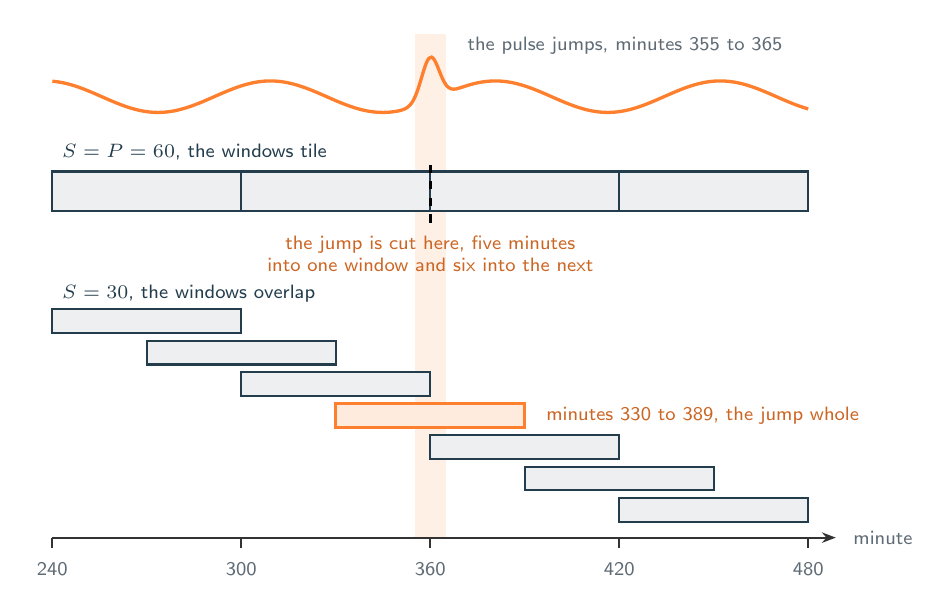
\begin{tikzpicture}[
    every node/.style={font=\sffamily},
    bar/.style={rectangle, draw=c2, fill=c2!8, line width=0.8pt},
    winbar/.style={rectangle, draw=c3, fill=c3!16, line width=1.2pt},
    lab/.style={font=\sffamily\scriptsize, text=labelcolor},
    tag/.style={font=\sffamily\scriptsize, text=c2},
    hot/.style={font=\sffamily\scriptsize, text=c3!80!black},
]

% the event, marked once and carried through the whole figure
\fill[c3!12] (5.40, 0.95) rectangle (5.80, 7.35);

% ============================================================ the signal
\draw[c3, line width=1.2pt]
    plot[domain=0.80:10.40, samples=280, smooth]
    (\x, {6.55 + 0.20*sin(\x r * 2.2) + 0.55*exp(-((\x-5.60)*(\x-5.60))/0.025)});
\node[lab, anchor=west] at (5.95, 7.20) {the pulse jumps, minutes 355 to 365};

% ============================================================ S = P = 60
\node[tag, anchor=west] at (0.80, 5.85) {$S = P = 60$, the windows tile};
\foreach \x/\n in {0.80/1, 3.20/2, 5.60/3, 8.00/4}{
    \draw[bar] (\x, 5.10) rectangle (\x+2.40, 5.60);
}
\draw[c1, line width=0.9pt, dashed] (5.60, 4.95) -- (5.60, 5.75);
\node[hot, anchor=north, align=center] at (5.60, 4.90)
    {the jump is cut here, five minutes\\ into one window and six into the next};

% ============================================================ S = 30
\node[tag, anchor=west] at (0.80, 4.05) {$S = 30$, the windows overlap};
\foreach \x/\y in {0.80/3.55, 2.00/3.15, 3.20/2.75, 5.60/1.95, 6.80/1.55, 8.00/1.15}{
    \draw[bar] (\x, \y) rectangle (\x+2.40, \y+0.30);
}
\draw[winbar] (4.40, 2.35) rectangle (6.80, 2.65);
\node[hot, anchor=west] at (6.95, 2.50) {minutes 330 to 389, the jump whole};

% ============================================================ time axis
\draw[axiscolor, line width=0.8pt, -{Stealth[length=5pt]}] (0.80, 0.95) -- (10.75, 0.95);
\foreach \x/\t in {0.80/240, 3.20/300, 5.60/360, 8.00/420, 10.40/480}{
    \draw[axiscolor, line width=0.7pt] (\x, 0.95) -- (\x, 0.82);
    \node[lab, anchor=north] at (\x, 0.76) {\t};
}
\node[lab, anchor=west] at (10.85, 0.95) {minute};

\end{tikzpicture}
\end{document}
